\fancyhead[L]{\textsf{\textbf{22}}\quad\textsf{\textbf{CHƯƠNG 1}}\quad\textsf{Hàm số và các mô hình}}
\fancyhead[R]{}

\noindent
\begin{minipage}[t]{0.26\textwidth}
    \vspace{5.58cm}
    \noindent
    \textbf{\textsf{HÌNH 1}}\\
    \textsf{\small Quá trình mô hình hóa}

    \vspace{2.95cm}
    \noindent
    \small
    \textsf{Hình học tọa độ của đường thẳng được ôn tập trong Phụ lục B.}

    \vspace{4.26cm}
    \noindent
    \textbf{\textsf{HÌNH 2}}
\end{minipage}%
\hfill
\begin{minipage}[t]{0.71\textwidth}
    \noindent
    kỹ năng toán học để tìm ra các phương trình liên hệ giữa các biến số. Trong những tình huống không có định luật vật lý nào định hướng, chúng ta có thể cần phải thu thập dữ liệu (từ Internet, từ thư viện hoặc bằng cách tự tiến hành các thí nghiệm) và khảo sát dữ liệu dưới dạng bảng nhằm phát hiện ra các quy luật. Từ biểu diễn dạng số này của một hàm số, chúng ta có thể muốn thu được một biểu diễn dạng đồ thị bằng cách vẽ các điểm dữ liệu. Trong một số trường hợp, đồ thị thậm chí còn có thể gợi ý cho ta một công thức đại số phù hợp.

    Giai đoạn thứ hai là áp dụng những kiến thức toán học mà chúng ta đã biết (chẳng hạn như phép tính vi tích phân sẽ được phát triển xuyên suốt cuốn sách này) vào mô hình toán học đã được thiết lập nhằm rút ra các kết luận toán học. Sau đó, ở giai đoạn thứ ba, chúng ta lấy những kết luận toán học đó và diễn giải chúng thành thông tin về hiện tượng thực tế ban đầu bằng cách đưa ra các lời giải thích hoặc dự đoán. Bước cuối cùng là kiểm tra các dự đoán của chúng ta bằng cách đối chiếu với dữ liệu thực tế mới. Nếu các dự đoán không phù hợp với thực tế, chúng ta cần hoàn thiện lại mô hình của mình hoặc xây dựng một mô hình mới và bắt đầu lại chu trình. Hình~1 minh họa cho quá trình mô hình hóa toán học.

    \vspace{0.25cm}
    \noindent
    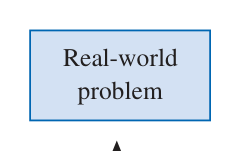
\includegraphics[width=\linewidth]{images/p0057_fig1.png}
    \vspace{0.16cm}

    Một mô hình toán học không bao giờ là sự mô tả chính xác hoàn toàn một tình huống vật lý---nó là một sự \emph{lý tưởng hóa}. Một mô hình tốt sẽ đơn giản hóa thực tế vừa đủ để cho phép thực hiện các tính toán toán học, nhưng cũng đủ chính xác để cung cấp các kết luận có giá trị. Điều quan trọng là phải nhận thức được những giới hạn của một mô hình.

    Có nhiều loại hàm số khác nhau có thể được sử dụng để mô hình hóa các mối quan hệ quan sát được trong thế giới thực. Dưới đây, chúng ta sẽ thảo luận về hành vi và đồ thị của một số hàm số này, đồng thời đưa ra các ví dụ về các tình huống được mô hình hóa một cách phù hợp bởi các hàm số đó.

    \vspace{0.33cm}
    \noindent
    {\color{stewartcyan}\rule{1.2ex}{1.2ex}}\;\textbf{\large\textsf{Mô hình tuyến tính}}
    \vspace{0.16cm}

    Khi nói rằng $y$ là một \textbf{hàm số tuyến tính} của $x$, chúng ta có ý nói rằng đồ thị của hàm số là một đường thẳng, do đó chúng ta có thể sử dụng phương trình đường thẳng dạng hệ số góc -- tung độ gốc để viết công thức cho hàm số dưới dạng
    \begin{equation*}
        y = f(x) = mx + b
    \end{equation*}
    trong đó $m$ là hệ số góc của đường thẳng và $b$ là tung độ gốc (giao điểm với trục tung).

    Một đặc điểm đặc trưng của các hàm số tuyến tính là chúng thay đổi với một tốc độ không đổi. Chẳng hạn, Hình~2 thể hiện đồ thị của hàm số tuyến tính $f(x) = 3x - 2$ và một bảng các giá trị mẫu. Chú ý rằng bất cứ khi nào $x$ tăng thêm $0{,}1$, giá trị của $f(x)$ lại tăng thêm $0{,}3$. Do đó $f(x)$ tăng nhanh gấp ba lần so với $x$. Điều này có nghĩa là hệ số góc của đồ thị $y = 3x - 2$, cụ thể là $3$, có thể được hiểu là tốc độ thay đổi của $y$ theo $x$.

    \vspace{0.33cm}
    \noindent
    \begin{minipage}[c]{0.52\linewidth}
        \centering
        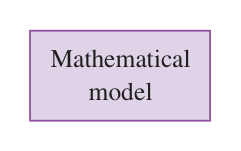
\includegraphics[width=0.9\linewidth]{images/p0057_fig2.png}
    \end{minipage}%
    \hfill
    \begin{minipage}[c]{0.45\linewidth}
        \centering
        \renewcommand{\arraystretch}{1.15}
        \begin{tabular}{|>{\centering\arraybackslash}p{1.4cm}|>{\centering\arraybackslash}p{2.4cm}|}
            \hline
            \rowcolor{stewartcyan!15} $x$ & $f(x) = 3x - 2$ \\
            \hline
            $1{,}0$ & $1{,}0$ \\
            $1{,}1$ & $1{,}3$ \\
            $1{,}2$ & $1{,}6$ \\
            $1{,}3$ & $1{,}9$ \\
            $1{,}4$ & $2{,}2$ \\
            $1{,}5$ & $2{,}5$ \\
            \hline
        \end{tabular}
    \end{minipage}
\end{minipage}